\doublespacing
\chapter{Another algorithmic improvement}
An algorithmic improvement can be applied to our algorithm. 
\section{Main Idea}
We notice that a large number of non-branching nodes exist in the tree representation of the RNA secondary structure. Therefore, we can construct compact representation for trees, which can aid in improving the running time for computing the tree edit distance. 
\section{Vertical Reduction on Trees}
Before we introduce the reduction on trees, it is benefit to define the compressible path on trees.
\begin{definition}
(Maximal Non-branching Path)A path in a tree is a non-branching path
if both the post-order tree traversal and pre-order tree traversal visit the nodes on the path in consecutive order. A non-branching path is maximal if no other non-branching path contains it ~\cite{Chen2014}.
\end{definition}

\begin{figure}
		\centering
		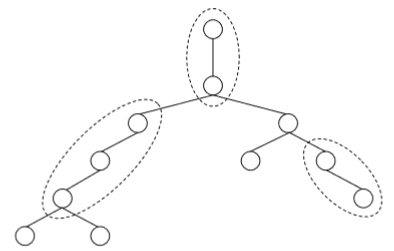
\includegraphics[width=6cm,clip]{Figures/VComponent}
		\label{Maximal Non-branching Path.} 
		\caption{Maximal non-branching path ~\cite{Chen2014}.}
\end{figure}
Figure 4.1 is an example of maximal non-branching path. Each maximal non-branching paths is enclosed by dashed line.

Each maximal non-branching paths is compressible, which gives rise to the vertical reduction.
\begin{definition}
(Vertical Reduction)
The vertical reduction on a tree is to replace every maximal non-branching path in the tree by a single node~\cite{Chen2014}.
\end{definition}

\begin{figure}
		\centering
		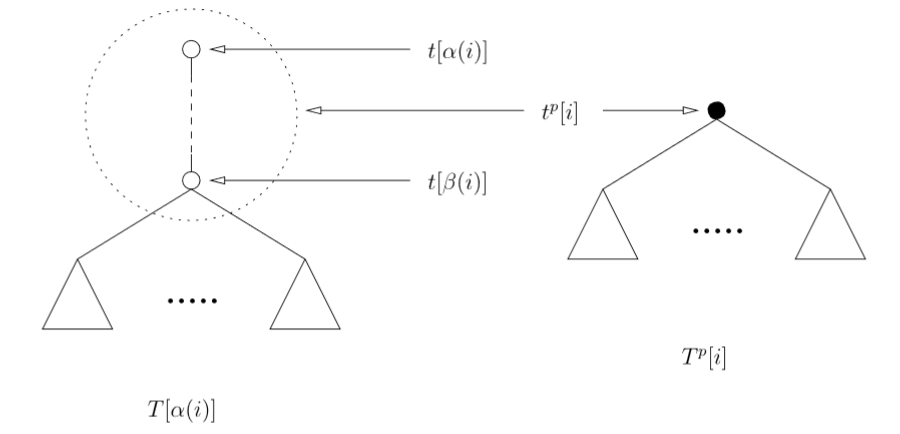
\includegraphics[width=10cm,clip]{Figures/VReduction}
		\label{An Example of the Mapping of Nodes Between the Original Tree and its Vertical Reduced Tree} 
		\caption{An example of the mapping of nodes between the original tree and its vertical reduced tree ~\cite{Chen2014}.}
\end{figure}

In Figure 4.2, we give an example of the mapping of nodes between the original tree(n the left) and its tree(on the right). Given a vertical reduced tree $\widetilde{T}$, two functions are respectively defined to map a node in compressed tree $\widetilde{t}[i]$ to the highest indexed node in the original tree $T$ $t[\alpha(i)]$ and the lowest indexed node $t[\beta(i)]$ of in the original tree $T$.  When $\widetilde(t)[i]$ corresponds to a single node in T, $t[\alpha(i)]=t[\beta(i)]$.

Please note that the compressed tree is just a compact representation of the original. Therefore, the strategy-based strategy in chapter 4 applied to the compressed tree can get the result same as that applied to the original tree. In other words, given trees $(T_1, T_2)$ and their reduced tree$(\widetilde{T_1}, \widetilde{T_2})$, the relation $d(\widetilde{T_1}, \widetilde{T_2}) = d(T_1, T_2)$ is implied. 

\section{Computation}

Following the Equation 2.3, let $\widetilde{F_1}$ and $\widetilde{F_2}$ be two relevant sub-forests in compressed trees,  $u$ and $v$ are nodes in forests $\widetilde{F_1}$ and $\widetilde{F_2}$ respectively, the forest-to-forest distance can be computed as follows:
\begin{equation}
d(\widetilde{F_1}, \widetilde{F_2}) = min \begin{cases}
d(\widetilde{F_1} - u, \widetilde{F_2}) + \delta(u, \varnothing) \\
d(\widetilde{F_1}, \widetilde{F_2} - v) + \delta(\varnothing, v) \\
d(\widetilde{F_1} - \widetilde{F_1(u)}, \widetilde{F_2} - \widetilde{F_2(v)}) + d(\widetilde{F_1(u)}, \widetilde{F_2(v)}) 
\end{cases}
\end{equation}
Each pairs of forest-forest distance $d(\widetilde{F_1}, \widetilde{F_2})$ can be computed correctly since each sub-problems has already been computed beforehand if implemented in post-order. The tree-tree distance, $d(\widetilde{F_1(u)}, \widetilde{F_2(v)})$, however, have never been computed before and must compute its value.

The tree-tree distance in compressed tree can be computed in the following lemmas.

\begin{lemma}
$d(\widetilde{F_1(i)}, \widetilde{F_2(j)}) = d(F_1(\alpha(i), F_2(\alpha(j))))$, where $i$ is a node in $\widetilde{F_1}$ and $j$ is a node in $\widetilde{F_2}$
\end{lemma}
\begin{proof}
The result follows from the compressed tree definition and the post-order implementation.
\end{proof}

To compute tree-to-tree distance of each sub-trees pairs in original trees, following Equation 2.2, we have Equation 4.2.

\begin{lemma}
$\forall u \in \{\beta(i), \cdots, \alpha(i)\}$ where $i$ is a node in $\widetilde{F_1}$, and $\forall v \in \{\beta(j), \cdots, \alpha(j)\}$ where $j$ is a node in $\widetilde{F_2}$.
\begin{equation}
d(F_1(u), F_2(v)) = min\begin{cases}
d(F_1^{\comp}(u), F_2(v)) + \delta(u, \varnothing)\\
d(F_1(u), F_2^{\comp}(v)) + \delta(\varnothing, v)\\
d(F_1^{\comp}(u), F_2^{\comp}(v)) + \delta(u, v)
\end{cases}
\end{equation}
\end{lemma}
\begin{proof}
The known recursive solution for the tree-to-tree edit distance.
\end{proof}

The computation of $d(F_1(u), F_2(v))$ involves sub-problems $d(F_1(u), F_2^{\comp}(\beta(j))), \forall u \in \{\beta(i), \cdots, \alpha(i)\}$ and $d(F_1^{\comp}(\beta(i)), F_2(v)), \forall v \in \{\beta(i), \cdots, \alpha(i)\}$ for the first time and therefore must compute their values beforehand. Therefore, initialization should be done to compute these values.  


\begin{lemma}
Let $F_2^{\comp}(\beta(j))$ be the form $F_2(j_1) \comp F_2(j_2) \cdots F_2(j_l)$, where $j \in \widetilde{F_2}$ and $j_1, j_2, \cdots, j_l$ be children of node $j$, $\forall u \in \{\beta(i), \cdots \alpha(i)\}$, where $i \in \widetilde{F_1}$,
\begin{equation}
d(F_1(u), F_2^{\comp}(\beta(j))) = min \begin{cases}
d(F_1^{\comp}(u), F_2^{\comp}(\beta(j))) + \delta(u, \varnothing)\\
min_{j_1' \leq q \leq j_l}\{d(F_1(u), F_2(\alpha(q))) - d(\varnothing, F_2(\alpha(q)))\} + d(\varnothing, F_2^{\comp}(\beta(j)))
\end{cases}
\end{equation}
\end{lemma}
\begin{proof}
The edit distance between tree $F_1(u)$ and the forest $F_2^{\comp}(\beta(j))$ consists of two possible cases. In the first case, $u$ is constrained to be deleted and the remaining substructure $F_1^{\comp}(u)$ is matched to $F_2^{\comp}(\beta(j))$. In the second case, $u$ is constrained to match a node somewhere in $F_2^{\comp}(\beta(j))$. In other words, tree $F_1(u)$ is matched to a sub-tree in $F_2^{\comp}(\beta(j))$. Therefore, the second case is finding a sub-tree in $F_2^{\comp}(\beta(j))$ to be matched to $F_1(u)$ so as to minimize $d(F_1(u), F_2^{\comp}(\beta(j)))$ under such constraint. 
\end{proof}

\begin{lemma}
Let $F_1^{\comp}(\beta(i))$ be the form $F_1(i_1) \comp F_1(i_2) \cdots F_1(i_k)$, where $i \in \widetilde{F_1}$ and $i_1, i_2, \cdots, i_l$ be children of node $i$, $\forall v \in \{\beta(j), \cdots \alpha(j)\}$, where $j \in \widetilde{F_2}$,
\begin{equation}
d(F_1^{\comp}(\beta(i)), F_2(v)) = min \begin{cases}
d(F_1^{\comp}(\beta(i)), F_2^{\comp}(v)) + \delta(\varnothing, v)\\
min_{i_1 \leq p \leq i_k}\{d(F_1(\alpha(p)), F_2(v)) - d(F_1(\alpha(p)), \varnothing)\} + d(F_1^{\comp}(\beta(i)), \varnothing)
\end{cases}
\end{equation}
\end{lemma}
\begin{proof}
The proof of Lemma 4.3.4 is symmetric to that of Lemma 4.3.3. The edit distance is the minimum value under two categories of constraints. 
\end{proof}

\section{Implementation}
The compressed tree is just a compact representation of the original. Thus, the algorithm is the same as in the Chapter 3:first find the optimal root-leaf path in compressed trees then compute distance in the bottom-up fashion. By Equation 4.1 and Lemma 4.3.1, 4.3.2, 4.3.3, the tree edit distance computation on compressed trees makes no differences to that on original trees when computing forest-to-forest distance but requires extra initialization steps when computing tree-to-tree distance. 

The tree-to-tree edit distance gives rise to five data structures. Let $T_1$ and $T_2$ be two original trees, while $\widetilde{T_1}$ and $\widetilde{T_2}$ be two compressed trees after vertical reductions on tree $T_1$ and $T_2$ respectively.
\begin{itemize}
\item $D_t$: a two dimensional permanent array of size $(\left\vert T_1 \right\vert + 1) * (\left\vert T_2 \right\vert + 1)$, which is used to store distance with respect to the $(T_1, T_2)$ representation.
\item $\widetilde{D_t}$: a two dimensional permanent array of size $(\left\vert \widetilde{T_1 }\right\vert + 1) * (\left\vert \widetilde{T_2} \right\vert + 1)$, which is used to store distances with respect to the $(\widetilde{T_1}, \widetilde{T_2})$ representation. 
\item $\widetilde{D_f}$: a two dimensional temporary array of size $(\left\vert \widetilde{T_1 }\right\vert + 1) * (\left\vert \widetilde{T_2} \right\vert + 1)$, which is used to store intermediate results for forest-to-forest distances.
\item $A_1, A_2$: temporary one dimensional arrays of lengths $(\left\vert T_1 \right\vert + 1)$ and $(\left\vert T_2 \right\vert + 1)$ respectively, which is used handle boundary initialization. 
\end{itemize}

We now present the algorithms to compute tree-to-tree edit distance on compressed trees. The algorithm details are shown in Algorithm 6. Let $\widetilde{A}$ and $\widetilde{B}$ be two compressed trees, $i \in \widetilde{A}$ and $j \in \widetilde{B}$.

\IncMargin{1em}
\begin{algorithm}
  \caption{TREE\_TO\_TREE\_DISTANCE}
  \SetKwData{TreeA}{$\widetilde{A(i)}$}
  \SetKwData{TreeB}{$\widetilde{B(j)}$}

  \For{$u \gets \beta(i) - 1$ \KwTo $\alpha(i)$} {
	$A_1[u] \gets D_t[u, \beta(j) - 1]$\;  
  }
  \For{$v \gets \beta(j)$ \KwTo $\alpha(j)$} {
	$A_2[v] \gets D_t[\beta(i) - 1, v]$\;  
  }
  $D_t[\beta(i) - 1, \beta(j) - 1] \gets \widetilde{D_f}[i - 1, j - 1]$\;
  \For{$u \gets \beta(i)$ \KwTo $\alpha(i)$} {
	$D_t[u, \beta(j) - 1] \gets min \begin{cases}
	D_t[u - 1, \beta(j) - 1] + \delta(A[u], \varnothing)\\
	min_{j_1 \leq q \leq j_l}\{D_t[u, \alpha(q)] - \sum_{k \in B(\alpha(q))}\delta(\varnothing, k)\} + \sum_{k \in B(\beta(j))}\delta(\varnothing, k)
	\end{cases}	
	$  
  }
  \For{$v \gets \beta(j)$ \KwTo $\alpha(j)$} {
  	$D_t[\beta(i) - 1, v] \gets min \begin{cases}
  	D_t[\beta(i) - 1, v - 1] + \delta(\varnothing, B[v])\\
  	min_{i_1 \leq p \leq i_k}\{D_t[\alpha(p), v] - \sum_{k \in A(\alpha(p))}\delta(k, \varnothing)+ \sum_{k \in A(\beta(i))}\delta(k, \varnothing)\}
	\end{cases}  	
  	$
  }
  \For{$u \gets \beta(i)$ \KwTo $\alpha(i)$} {
	\For{$v \gets \beta(j)$ \KwTo $\alpha(j)$} {
		$D_t[u, v] \gets min \begin{cases}
		D_t[u - 1, v] + \delta(u, \varnothing)\\
		D_t[u, v - 1] + \delta(\varnothing, v)\\
		D_t[u - 1, v - 1] + \delta(u, v)
		\end{cases}		
		$	
	} 
  }
  $\widetilde{D_t}[i, j] \gets D_t[\alpha(i), \alpha(j)]$\;
  $\widetilde{D_f}[i, j] \gets D_t[\alpha(i), \alpha(j)]$\;
  \For{$u \gets \beta(i) - 1$ \KwTo $\alpha(i)$}{
  	$D_t[u, \beta(j) - 1] \gets A_1[u]$\;
  }
  \For{$v \gets \beta(j)$ \KwTo $\alpha(j)$} {
	$D_t[\beta(i) - 1, v] \gets A_2[v]$\;  
  }
\end{algorithm}

The algorithm of forest-to-forest edit distance on compressed trees is the exactly the same as that on original trees, using Equation 3.1 or 3.2 depending on the decomposition directions. The details of the forest-to-forest edit distance computation is shown in Algorithm 7 and 8.

\IncMargin{1em}
\begin{algorithm}
  \caption{FOREST\_TO\_FOREST\_DISTANCE}
  \SetKwData{TreeA}{$\widetilde{A(i)}$}
  \SetKwData{TreeB}{$\widetilde{B(j)}$}
  $sizelA \gets$ the size of A(lA)\;
  $sizelB \gets$ the size of B(lB)\;
  $\widetilde{D_f}[lA, lB] \gets min \begin{cases}
	\widetilde{D_f}[lA - 1, lB] + \delta(lA, \varnothing)\\
	\widetilde{D_f}[lA, lB - 1] + \delta(\varnothing, lB)\\
	\widetilde{D_f}[lA - sizelA, lB - sizelB] + \widetilde{D_t}[lA, lB]
  \end{cases}  
  $
\end{algorithm}

\IncMargin{1em}
\begin{algorithm}
  \caption{FOREST\_TO\_FOREST\_DISTANCE}
  \SetKwData{TreeA}{$\widetilde{A(i)}$}
  \SetKwData{TreeB}{$\widetilde{B(j)}$}
  $sizerA \gets$ the size of A(rA)\;
  $sizerB \gets$ the size of B(rB)\;
  $\widetilde{D_f}[rA, rB] \gets min \begin{cases}
	\widetilde{D_f}[rA - 1, rB] + \delta(rA, \varnothing)\\
	\widetilde{D_f}[rA, rB - 1] + \delta(\varnothing, rB)\\
	\widetilde{D_f}[rA - sizerA, lB - sizerB] + \widetilde{D_t}[rA, rB]
  \end{cases}  
  $
\end{algorithm}